\documentclass[12pt,letterpaper]{article}
\usepackage{graphicx,textcomp}
\usepackage{natbib}
\usepackage{setspace}
\usepackage{fullpage}
\usepackage{color}
\usepackage[reqno]{amsmath}
\usepackage{amsthm}
\usepackage{fancyvrb}
\usepackage{amssymb,enumerate}
\usepackage[all]{xy}
\usepackage{endnotes}
\usepackage{lscape}
\newtheorem{com}{Comment}
\usepackage{float}
\usepackage{hyperref}
\newtheorem{lem} {Lemma}
\newtheorem{prop}{Proposition}
\newtheorem{thm}{Theorem}
\newtheorem{defn}{Definition}
\newtheorem{cor}{Corollary}
\newtheorem{obs}{Observation}
\usepackage[compact]{titlesec}
\usepackage{dcolumn}
\usepackage{tikz}
\usetikzlibrary{arrows}
\usepackage{multirow}
\usepackage{xcolor}
\newcolumntype{.}{D{.}{.}{-1}}
\newcolumntype{d}[1]{D{.}{.}{#1}}
\definecolor{light-gray}{gray}{0.65}
\usepackage{url}
\usepackage{listings}
\usepackage{color}

\definecolor{codegreen}{rgb}{0,0.6,0}
\definecolor{codegray}{rgb}{0.5,0.5,0.5}
\definecolor{codepurple}{rgb}{0.58,0,0.82}
\definecolor{backcolour}{rgb}{0.95,0.95,0.92}

\lstdefinestyle{mystyle}{
	backgroundcolor=\color{backcolour},   
	commentstyle=\color{codegreen},
	keywordstyle=\color{magenta},
	numberstyle=\tiny\color{codegray},
	stringstyle=\color{codepurple},
	basicstyle=\footnotesize,
	breakatwhitespace=false,         
	breaklines=true,                 
	captionpos=b,                    
	keepspaces=true,                 
	numbers=left,                    
	numbersep=5pt,                  
	showspaces=false,                
	showstringspaces=false,
	showtabs=false,                  
	tabsize=2
}
\lstset{style=mystyle}
\newcommand{\Sref}[1]{Section~\ref{#1}}
\newtheorem{hyp}{Hypothesis}

\title{Problem Set 3}
\date{Due: November 19, 2022}
\author{Applied Stats/Quant Methods 1}


\begin{document}
	\maketitle
	\section*{Instructions}
	\begin{itemize}
		\item Please show your work! You may lose points by simply writing in the answer. If the problem requires you to execute commands in \texttt{R}, please include the code you used to get your answers. Please also include the \texttt{.R} file that contains your code. If you are not sure if work needs to be shown for a particular problem, please ask.
	\item Your homework should be submitted electronically on GitHub.
	\item This problem set is due before 23:59 on Sunday November 19, 2023. No late assignments will be accepted.

	\end{itemize}

		\vspace{.25cm}
	
\noindent In this problem set, you will run several regressions and create an add variable plot (see the lecture slides) in \texttt{R} using the \texttt{incumbents\_subset.csv} dataset. Include all of your code.

	\vspace{.5cm}
\section*{Question 1}
\vspace{.25cm}
\noindent We are interested in knowing how the difference in campaign spending between incumbent and challenger affects the incumbent's vote share. 

	\begin{enumerate}
		\item Run a regression where the outcome variable is \texttt{voteshare} and the explanatory variable is \texttt{difflog}.	\vspace{0.05cm}
		
							\vspace{.05cm}
		\lstinputlisting[language=R, firstline=89, lastline=94]{/Users/iseli/Documents/GitHub/StatsI_Fall2023/problemSets/PS03/my_answers/PS3.R}  
		\begin{footnotesize}
			
			\begin{verbatim}
				Call:
				lm(formula = voteshare ~ difflog, data = inc.sub)
				  
				Residuals:
				Min       1Q   					Median       3Q      Max  
				-0.26832 -0.05345 -0.00377  0.04780  0.32749 
				
				Coefficients:
				Estimate Std. Error t value Pr(>|t|)    
				(Intercept)   0.579031   0.002251  257.19   <2e-16 ***
				difflog       0.041666   0.000968   43.04   <2e-16 ***  
				---
				Signif. codes:  0 ‘***’ 0.001 ‘**’ 0.01 ‘*’ 0.05 ‘.’ 0.1 ‘ ’ 1
				Residual standard error: 0.07867 on 3191 degrees of freedom
				Multiple R-squared:  0.3673,	Adjusted R-squared:  0.3671
				F-statistic: 1853 on 1 and 3191 DF,  p-value: < 2.2e-16
			\end{verbatim}
		\end{footnotesize}
	
		\vspace{0.05cm}
		\item Make a scatterplot of the two variables and add the regression line. 	\vspace{0.05cm}
			\begin{lstlisting}[language=R]
				# Dataset
				inc.sub <- read.csv("https://raw.githubusercontent.com/ASDS-TCD/StatsI_Fall2023/main/datasets/incumbents_subset.csv")
				
				# Make a scatterplot of the two variables and add the regression line
				plot(inc.sub$difflog, inc.sub$voteshare, main="Scatterplot of difflog and voteshare with Regression Line")
				abline(lm_model, col="red")
			\end{lstlisting}			
	\vspace{0.05cm}
	\begin{figure}[h!]
		\centering
		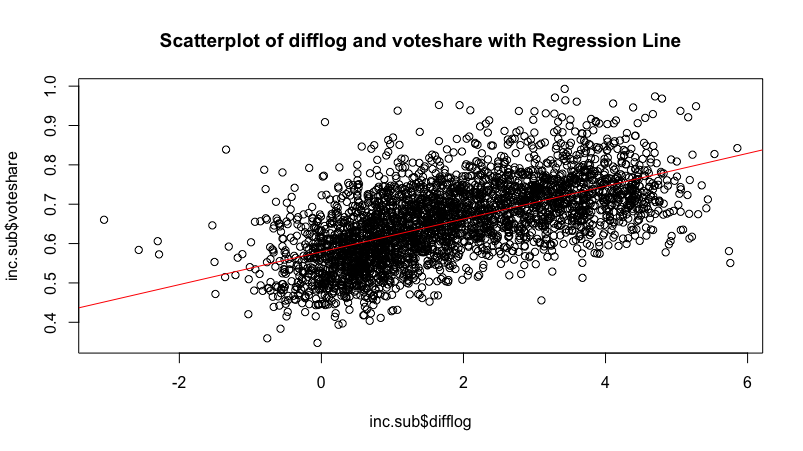
\includegraphics[width=0.8\textwidth]{/Users/iseli/Documents/GitHub/StatsI_Fall2023/problemSets/PS03/my_answers/Rplot 1.png}
		\caption{Scatterplot of difflog and voteshare with Regression Line}
		\label{fig:scatterplot}
	\end{figure}


	\item Save the residuals of the model in a separate object.
	\vspace{0.05cm}
	
				\begin{verbatim}
			Call:
			lm(formula = voteshare ~ difflog, data = inc.sub)
		
			Residuals:
			Min       1Q   					Median       3Q      Max  
			-0.26832 -0.05345 -0.00377  0.04780  0.32749 
				\end{verbatim}
	
	
	\item Write the prediction equation.
	\vspace{0.05cm}	
	
				\begin{verbatim}
		Coefficients:
		Estimate Std. Error t value Pr(>|t|)    
		(Intercept)   0.579031   0.002251  257.19   <2e-16 ***
		difflog       0.041666   0.000968   43.04   <2e-16 ***
		---
		Signif. codes:  0 ‘***’ 0.001 ‘**’ 0.01 ‘*’ 0.05 ‘.’ 0.1 ‘ ’ 1
		Residual standard error: 0.07867 on 3191 degrees of freedom
		Multiple R-squared:  0.3673,	Adjusted R-squared:  0.3671 
		F-statistic: 1853 on 1 and 3191 DF,  p-value: < 2.2e-16
	\end{verbatim}
	
\end{enumerate}			

\section*{Question 2}
\noindent We are interested in knowing how the difference between incumbent and challenger's spending and the vote share of the presidential candidate of the incumbent's party are related.	\vspace{.25cm}
	\begin{enumerate}
		\item Run a regression where the outcome variable is \texttt{presvote} and the explanatory variable is \texttt{difflog}.	\vspace{0.05cm}
		
					\begin{verbatim}
			Call:
			lm(formula = presvote ~ difflog, data = inc.sub)
			
			Residuals:
			Min       1Q   					Median       3Q      Max  
			-0.32196 -0.07407 -0.00102  0.07151  0.42743 
			
			Coefficients:
			Estimate Std. Error t value Pr(>|t|)    
			(Intercept)   0.507583   0.003161  160.60   <2e-16 ***
			difflog       0.023837   0.001359   17.54   <2e-16 ***
			---
			Signif. codes:  0 ‘***’ 0.001 ‘**’ 0.01 ‘*’ 0.05 ‘.’ 0.1 ‘ ’ 1
			Residual standard error: 0.1104 on 3191 degrees of freedom
			Multiple R-squared:  0.08795,	Adjusted R-squared:  0.08767
			F-statistic: 307.7 on 1 and 3191 DF,  p-value: < 2.2e-16
				\end{verbatim}
	\newpage			
		\item Make a scatterplot of the two variables and add the regression line. 	\vspace{0.05cm}
			\begin{lstlisting}[language=R]
			# Dataset
			inc.sub <- read.csv("https://raw.githubusercontent.com/ASDS-TCD/StatsI_Fall2023/main/datasets/incumbents_subset.csv")
			
			# Make a scatterplot of the two variables and add the regression line
			plot(inc.sub$difflog, inc.sub$presvote, main="Scatterplot of difflog and presvote with Regression Line")abline(lm_model, col="red")
		\end{lstlisting}			
		\vspace{0.05cm}
		\begin{figure}[h!]
			\centering
			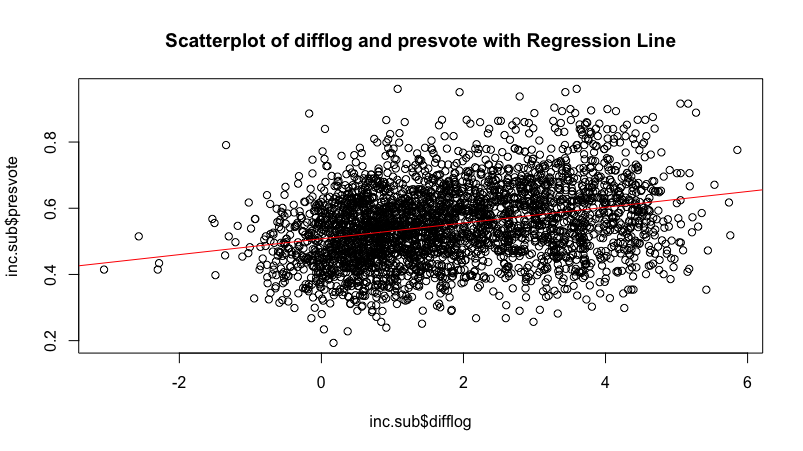
\includegraphics[width=0.8\textwidth]{/Users/iseli/Documents/GitHub/StatsI_Fall2023/problemSets/PS03/my_answers/Rplot 2.png}
			\caption{Scatterplot of difflog and presvote with Regression Line}
			\label{fig:scatterplot difflog and presvote}
		\end{figure}
		
		\item Save the residuals of the model in a separate object.	\vspace{0.05cm}
			\vspace{0.05cm}
		
		\begin{verbatim}
			Call:
			lm(formula = presvote ~ difflog, data = inc.sub)
			
			Residuals:
			Min       1Q   					Median       3Q      Max  
			-0.32196 -0.07407 -0.00102  0.07151  0.42743 
		\end{verbatim}
		
		\item Write the prediction equation.
			\vspace{0.05cm}	
		\begin{verbatim}
			Coefficients:
			Estimate Std. Error t value Pr(>|t|)    
			(Intercept)   0.507583   0.003161  160.60   <2e-16 ***
			difflog       0.023837   0.001359   17.54   <2e-16 ***
			---
			Signif. codes:  0 ‘***’ 0.001 ‘**’ 0.01 ‘*’ 0.05 ‘.’ 0.1 ‘ ’ 1
			Residual standard error: 0.1104 on 3191 degrees of freedom
			Multiple R-squared:  0.08795,	Adjusted R-squared:  0.08767 
			F-statistic: 307.7 on 1 and 3191 DF,  p-value: < 2.2e-16
		\end{verbatim}
		
	\end{enumerate}
	
\section*{Question 3}

\noindent We are interested in knowing how the vote share of the presidential candidate of the incumbent's party is associated with the incumbent's electoral success.
	\vspace{.25cm}
	\begin{enumerate}
		\item Run a regression where the outcome variable is \texttt{voteshare} and the explanatory variable is \texttt{presvote}.
			\vspace{0.05cm}
			
				\begin{verbatim}
				Call:
				lm(formula = voteshare ~ presvote, data = inc.sub)
				
				Residuals:
				Min       1Q   					Median       3Q      Max  
				-0.27330 -0.05888  0.00394  0.06148  0.41365 
				
				Coefficients:
				Estimate Std. Error t value Pr(>|t|)    
				(Intercept)   0.441330   0.007599   58.08   <2e-16 ***
				presvote       0.441330   0.007599   58.08   <2e-16 ***
				---
				Signif. codes:  0 ‘***’ 0.001 ‘**’ 0.01 ‘*’ 0.05 ‘.’ 0.1 ‘ ’ 1
				Residual standard error: 0.08815 on 3191 degrees of freedom
				Multiple R-squared:  0.2058,	Adjusted R-squared:  0.2056 
				F-statistic: 827 on 1 and 3191 DF,  p-value: < 2.2e-16
			\end{verbatim}
			
		\item Make a scatterplot of the two variables and add the regression line. 
			\begin{lstlisting}[language=R]
			# Dataset
			inc.sub <- read.csv("https://raw.githubusercontent.com/ASDS-TCD/StatsI_Fall2023/main/datasets/incumbents_subset.csv")
			
			# Make a scatterplot of the two variables and add the regression line
			plot(inc.sub$presvote, inc.sub$voteshare, main="Scatterplot of presvote and voteshare with Regression Line")abline(lm_model, col="red")
				\end{enumerate}
		\end{lstlisting}			
		\vspace{0.05cm}
		\begin{figure}[h!]
			\centering
			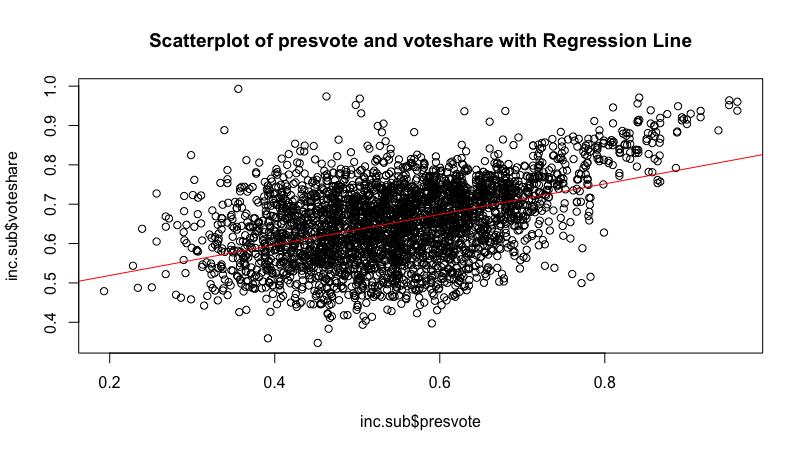
\includegraphics[width=0.8\textwidth]{/Users/iseli/Documents/GitHub/StatsI_Fall2023/problemSets/PS03/my_answers/Rplot 3.png}
			\caption{Scatterplot of voteshare and presvote with Regression Line}
			\label{fig:scatterplot voteshare and presvote}
		\end{figure}
		
			\vspace{0.05cm}
		\item Write the prediction equation.

					\begin{verbatim}		
		Coefficients:
		Estimate Std. Error t value Pr(>|t|)    
		(Intercept)   0.441330   0.007599   58.08   <2e-16 ***
		presvote       0.441330   0.007599   58.08   <2e-16 ***
		---
		Signif. codes:  0 ‘***’ 0.001 ‘**’ 0.01 ‘*’ 0.05 ‘.’ 0.1 ‘ ’ 1
		Residual standard error: 0.08815 on 3191 degrees of freedom
		Multiple R-squared:  0.2058,	Adjusted R-squared:  0.2056 
		F-statistic: 827 on 1 and 3191 DF,  p-value: < 2.2e-16
	\end{verbatim}

\section*{Question 4}
\noindent The residuals from part (a) tell us how much of the variation in \texttt{voteshare} is $not$ explained by the difference in spending between incumbent and challenger. The residuals in part (b) tell us how much of the variation in \texttt{presvote} is $not$ explained by the difference in spending between incumbent and challenger in the district.
	\begin{enumerate}
		\item Run a regression where the outcome variable is the residuals from Question 1 and the explanatory variable is the residuals from Question 2.	\vspace{0.05cm}
		
			\begin{verbatim}
			Call:
			lm(formula = residuals_question1 ~ residuals_question2)
			
			Residuals:
			1			        	2   											3       				4      								5  
			-0.008079  0.011143  0.003168 -0.002506 -0.003727  
			
			Coefficients:
			Estimate Std. Error t value Pr(>|t|)    
			(Intercept)   -0.006133   0.003840  -1.597    0.209 
			residuals_question2       0.789254   0.015757  50.088 1.75e-05 ***
			---
			Signif. codes:  0 ‘***’ 0.001 ‘**’ 0.01 ‘*’ 0.05 ‘.’ 0.1 ‘ ’ 1
			Residual standard error: 0.008557 on 3 degrees of freedom
			Multiple R-squared:  0.9988,	Adjusted R-squared:  0.9984 
			F-statistic: 2509 on 1 and 3 DF,  p-value: 1.752e-05
		\end{verbatim}
		
		\item Make a scatterplot of the two residuals and add the regression line. 	\vspace{0.05cm}
		
					\begin{lstlisting}[language=R]
			# Dataset
			inc.sub <- read.csv("https://raw.githubusercontent.com/ASDS-TCD/StatsI_Fall2023/main/datasets/incumbents_subset.csv")
			
			# Make a scatterplot of the two variables and add the regression line
			plot(residuals_question2, residuals_question1, main="Scatterplot of Residuals from Question 2 and Question 1 with Regression Line")abline(lm_model_residuals, col="red")
		\end{enumerate}
		\end{lstlisting}			
		\vspace{0.05cm}
		\begin{figure}[h!]
		\centering
		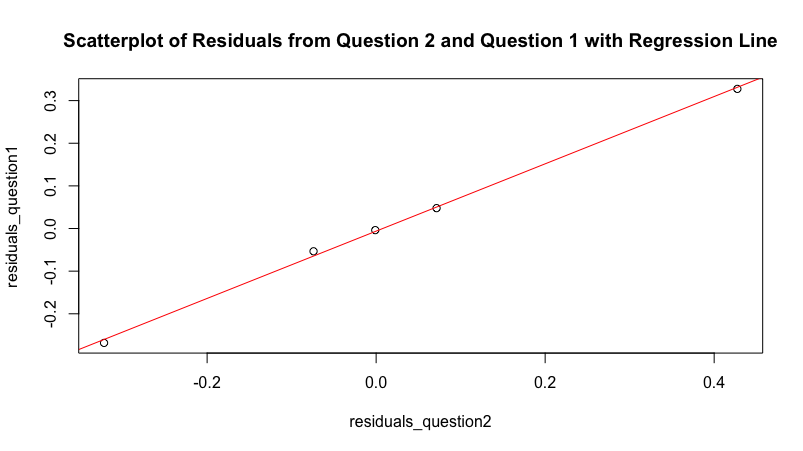
\includegraphics[width=0.8\textwidth]{/Users/iseli/Documents/GitHub/StatsI_Fall2023/problemSets/PS03/my_answers/Rplot 4.png}
		\caption{Scatterplot of Residuals Q1 and Residuals Q2 with Regression Line}
		\label{fig:scatterplot residuals q1 and residuals q2}
		\end{figure}
		
		\vspace{0.05cm}
		
		\item Write the prediction equation.
					\begin{verbatim}			
			Coefficients:
			Estimate Std. Error t value Pr(>|t|)    
			(Intercept)   -0.006133   0.003840  -1.597    0.209 
			residuals_question2       0.789254   0.015757  50.088 1.75e-05 ***
			---
			Signif. codes:  0 ‘***’ 0.001 ‘**’ 0.01 ‘*’ 0.05 ‘.’ 0.1 ‘ ’ 1
			Residual standard error: 0.008557 on 3 degrees of freedom
			Multiple R-squared:  0.9988,	Adjusted R-squared:  0.9984 
			F-statistic: 2509 on 1 and 3 DF,  p-value: 1.752e-05
		\end{verbatim}
		
	\end{enumerate}

\section*{Question 5}
\noindent What if the incumbent's vote share is affected by both the president's popularity and the difference in spending between incumbent and challenger? 
	\begin{enumerate}
		\item Run a regression where the outcome variable is the incumbent's \texttt{voteshare} and the explanatory variables are \texttt{difflog} and \texttt{presvote}.	\vspace{0.05cm}
		
					\begin{verbatim}
			Call:
			lm_model <- lm(voteshare ~ difflog + presvote, data = inc.sub)
		\end{verbatim}
		
		\item Write the prediction equation.	\vspace{0.05cm}
		
					\begin{verbatim}
			Call:
			lm(formula = voteshare ~ difflog + presvote, data = inc.sub)
			
			Residuals:
			Min       1Q   Median       3Q      Max  
			-0.25928 -0.04737 -0.00121  0.04618  0.33126
			
			Coefficients:
			Estimate Std. Error t value Pr(>|t|)    
			(Intercept)   0.4486442  0.0063297   70.88   <2e-16 ***
			difflog       0.0355431  0.0009455   37.59   <2e-16 ***
			presvote       0.2568770  0.0117637   21.84   <2e-16 ***
			---
			Signif. codes:  0 ‘***’ 0.001 ‘**’ 0.01 ‘*’ 0.05 ‘.’ 0.1 ‘ ’ 1
			Residual standard error: 0.07339 on 3190 degrees of freedom
			Multiple R-squared:  0.4496,	Adjusted R-squared:  0.4493
			F-statistic: 1303 on 2 and 3190 DF,  p-value: < 2.2e-16
		\end{verbatim}
		
		\item What is it in this output that is identical to the output in Question 4? Why do you think this is the case?
		
		The reason, for this similarity is that both Question 4 and Question 5 have the intention of examining how various factors affect the variable. They achieve this by taking into account the variation through the use of residuals from models. By incorporating these residuals as variables in regressions we can determine to what extent additional factors beyond those initially considered in the models contribute to explaining the remaining variation, in the dependent variable. This approach provides a understanding of the factors that influence the dependent variable.
		
	\end{enumerate}
\end{document}
